\documentclass[
    11pt,
    a4paper,
    sfdefaults=false,
    toc=chapterentrywithdots,
    %twoside,openright,
    oneside,openright,
    titlepage,
    parskip=half,
    headings=normal,  % reduces heading size
    listof=totoc,
    bibliography=totoc,
    index=totoc,
    captions=tableheading,  % caption below table
    %chapterprefix,
    listof=flat,
    final
]{scrbook}

\RedeclareSectionCommand[
  beforeskip=0mm, 
  afterskip=0mm    
]{chapter}

\RedeclareSectionCommand[
  beforeskip=0mm, 
  afterskip=1mm    
]{section}

% details about your thesis
\newcommand{\titel}{Modellierung und Simulation eines Doppelpendels und Dreifachpendels}
\newcommand{\artderarbeit}{Studienarbeit}
\newcommand{\untertitel}{für Modellbildung und Simulation}
\newcommand{\autor}{Changlai Bao}
\newcommand{\studiengang}{Elektronische und Mechatronische Systeme}
\newcommand{\matrikelnr}{3834688}
\newcommand{\keywords}{hot, fuzz}

% custom head and foot
\usepackage[automark]{scrlayer-scrpage}
\pagestyle{scrheadings}
\ihead{\headmark}
\chead{}
\ohead{\pagemark}
\renewcommand*\chaptermarkformat{\chapappifchapterprefix{\ }% 
\thechapter.\enskip}

\KOMAoption{headsepline}{true} % Linie unter Kopfzeile 
\KOMAoption{footsepline}{true} % Linie über Fußzeile
\addtokomafont{headsepline}{\color{red!80!black}}
\addtokomafont{footsepline}{\color{red!80!black}} 

\renewcommand*{\chapterpagestyle}{scrheadings} % Kopfzeile auf Kapitelseiten
\cfoot*{\pagemark} % Seitenzahl in der Mitte der Fußzeile

\RedeclareSectionCommand[tocindent=0pt]{section}
\RedeclareSectionCommand[tocindent=0pt]{subsection}
%\RedeclareSectionCommand[tocnumwidth=70pt]{chapter}

\usepackage{scrhack}

% other packages
\usepackage[utf8]{inputenc}
\usepackage[T1]{fontenc}
\usepackage{lmodern,relsize,textcomp,csquotes}
\usepackage{amsmath,amsfonts}
\usepackage[english, ngerman]{babel}  % flip for German thesis
\usepackage[final]{graphicx}
\usepackage{setspace,geometry,xcolor}
\usepackage{makeidx}
\usepackage{paralist,ifthen,todonotes}
\usepackage{url}
\usepackage[toc]{glossaries}
\usepackage{pdfpages}
\usepackage{float}
\usepackage{subcaption}

% table setup
\usepackage{longtable}
\usepackage{array}
\usepackage{ragged2e}
\usepackage{lscape}

% pdf hyperref
\usepackage[
    bookmarks=true,
    bookmarksopen=true,
    bookmarksnumbered=true,
    bookmarksopenlevel=1,
    pdftitle={\titel},
    pdfauthor={\autor},
    pdfcreator={\autor},
    pdfsubject={\titel},
    pdfkeywords={\keywords},
    pdfpagelabels=true,
    colorlinks=true,
    linkcolor={red!80!black},
    urlcolor=magenta,
    anchorcolor=black,
    citecolor=cyan,
    filecolor=magenta,
    menucolor=red,
    plainpages=false,
    hypertexnames=true,
    linktocpage=true,
]{hyperref}

% configure your listings style
\usepackage{listings}
\lstset{
    tabsize=3,
    extendedchars=true,
    frame=single,
    showstringspaces=true,
    numbers=left,
    numberstyle=\small,
    breakautoindent=true,
    breaklines=true,
    commentstyle=\color{green!60!black},
    keywordstyle=\color{blue},
    stringstyle=\color{purple},
    basicstyle=\ttfamily\small,
    language=Matlab
}

% configure your glossaries
\usepackage{tcolorbox}
\tcbuselibrary{most}
\newtcbox{\codefile}{
  enhanced,
  nobeforeafter,
  tcbox raise base,
  boxrule=0.4pt,
  arc=4pt,
  fontupper=\ttfamily\small\color{black}, 
  colback=orange!30,
  colframe=orange!70!black, 
  top=0pt,
  bottom=0pt,
  left=3pt,
  right=3pt,
  boxsep=0pt,
  height=2.5ex,
  valign=center
}

% page setup
% \setlength{\topskip}{\ht\strutbox}
\geometry{paper=a4paper,left=2.5cm,top=3.0cm,bindingoffset=.8cm}
\onehalfspacing
\frenchspacing
\clubpenalty = 10000
\widowpenalty = 10000 
\displaywidowpenalty = 10000
\sloppy

% some commands
\newcommand{\ua}{\mbox{u.\,a.\ }}
\newcommand{\zB}{\mbox{z.\,B.\ }}
\newcommand{\dahe}{\mbox{d.\,h.,\ }}
\newcommand{\bzw}{\mbox{bzw.\ }}
\newcommand{\bzgl}{\mbox{bzgl.\ }}
\newcommand{\eg}{\mbox{e.\,g.\ }}
\newcommand{\ie}{\mbox{i.\,e.\ }}
\newcommand{\wrt}{\mbox{w.\,r.\,t.\ }}
\newcommand{\etal}{\mbox{\emph{et\,al.\ }}}


% TODO remove if not needed...
\usepackage{blindtext}

\begin{document}

\setcounter{secnumdepth}{3}  % numerate subsections
\setcounter{tocdepth}{2}  % ...but don't include them in toc

\frontmatter
\thispagestyle{empty}
\pdfbookmark[1]{Cover}{cov}
\begin{titlepage}

\begin{center}


\includegraphics[width=0.9\linewidth]{figures/efi-logo.jpg}\\[2cm]

\huge
\textbf{\titel}\\[1cm]

\vspace*{\fill}

\LARGE
\textbf{\artderarbeit}\\[0.5cm]

\Large
\textbf{\untertitel}\\[1cm]

\Large 
~im Studiengang \studiengang\\[1cm]

\vspace*{\fill}

\Large
Autor: \autor\\[0.5cm]

\Large
Matrikelnummer: \matrikelnr\\[2cm]

\end{center}

\begin{center}
\copyright\,\the\year
\end{center}

\end{titlepage}


% download the following form (requires VPN) and complete it (hit save in your editor)
% https://intern.ohmportal.de/fileadmin/Public_Docs/SB/SB_0009_FO_Pruefungsrechtliche_Erklaerung_und_Erklaerung_zur_Veroeffentlichung_der_Abschlussarbeit_public.pdf
%\includepdf{SB_0009_FO_Pruefungsrechtliche_Erklaerung_und_Erklaerung_zur_Veroeffentlichung_der_Abschlussarbeit_public.pdf}\cleardoublepage

\setcounter{page}{1}
%\tableofcontents

\mainmatter
\chapter{Beschreibung des Systems}\label{ch:Systembeschreibung}
Diese Arbeit beschäftigt sich mit der Modellierung und Simulation eines Doppelpendels und eines Dreifachpendels. 

Das Doppelpendel besteht aus zwei Pendeln, die an einem gemeinsamen Punkt aufgehängt sind. Die Abbildung \ref{fig:Doppelpendel} zeigt das System mit den relevanten Größen. Die Längen $l_1$ und $l_2$ der Pendelarme sowie die Massen $m_1$ und $m_2$ der Pendel sind dargestellt. Die Abbildung zeigt auch die Abstände $s_1$ und $s_2$, die die Abstände der Massen von den Aufhängepunkten beschreiben. Die Gravitationskonstante $g$ und die Trägheitsmomente $J_1$ und $J_2$ der Pendel sind ebenfalls angegeben. Außerdem sind die Winkel $\varphi_1$ und $\varphi_2$ eingezeichnet, die die Lage der Pendel relativ zur Vertikalen beschreiben. Die Abbildung zeigt auch die Positionen $x_1$, $y_1$, $x_2$ und $y_2$, die die Endpunkte der Pendel darstellen. 

Das Dreifachpendel besteht aus drei Pendeln, die ebenfalls an einem gemeinsamen Punkt aufgehängt sind. Die Abbildung \ref{fig:Dreifachpendel} zeigt das System mit den relevanten Größen. Die Längen $l_1$, $l_2$ und $l_3$ der Pendelarme sowie die Massen $m_1$, $m_2$ und $m_3$ der Pendel sind dargestellt. Die Abbildung zeigt auch die Abstände $s_1$, $s_2$ und $s_3$, die die Abstände der Massen von den Aufhängepunkten beschreiben. Die Gravitationskonstante $g$ und die Trägheitsmomente $J_1$, $J_2$ und $J_3$ der Pendel sind ebenfalls angegeben. Außerdem sind die Winkel $\varphi_1$, $\varphi_2$ und $\varphi_3$ eingezeichnet, die die Lage der Pendel relativ zur Vertikalen beschreiben. Die Abbildung zeigt auch die Positionen $x_1$, $y_1$, $x_2$, $y_2$, $x_3$ und $y_3$, die die Endpunkte der Pendel darstellen.

\begin{figure}[H]
  \centering
  \begin{subfigure}{0.47\textwidth}
    \centering
    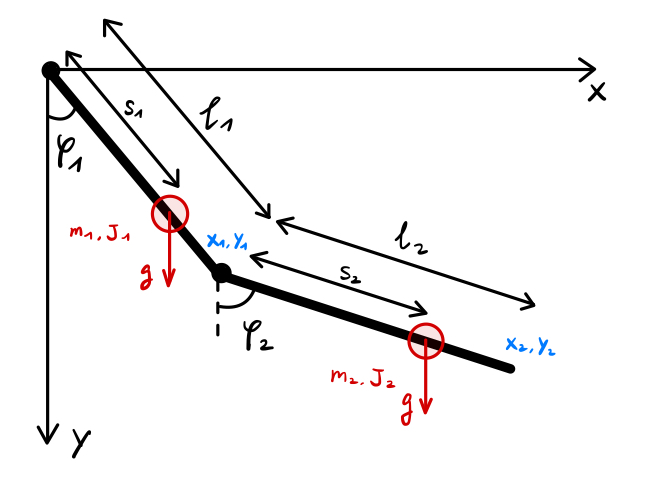
\includegraphics[width=\textwidth]{figures/Doppelpendel.png}
    \caption{Doppelpendel}
    \label{fig:Doppelpendel}
  \end{subfigure}
  \hfill 
  \begin{subfigure}{0.51\textwidth}
    \centering
    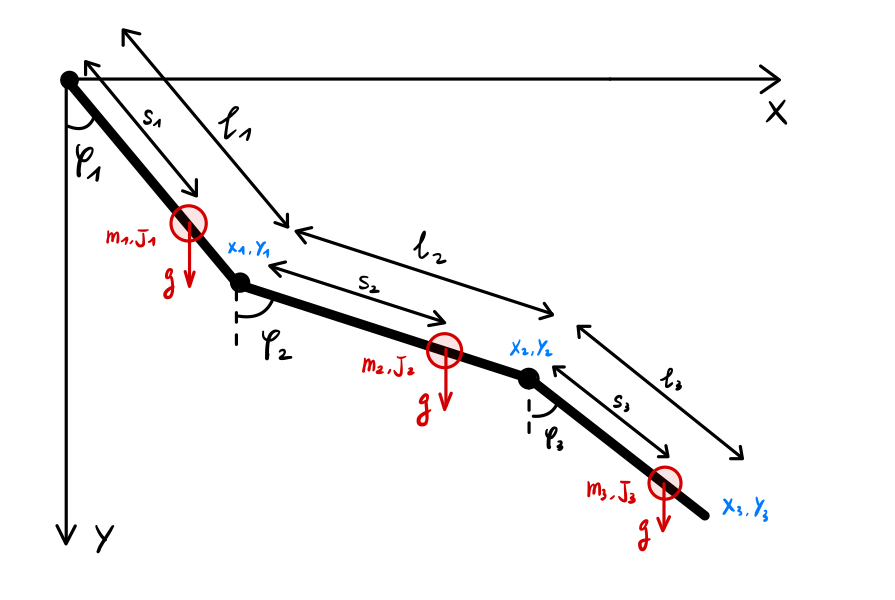
\includegraphics[width=\textwidth]{figures/Dreifachpendel.png}
    \caption{Dreifachpendel}
    \label{fig:Dreifachpendel}
  \end{subfigure}
  \caption{Doppelpendel und Dreifachpendel}
  \label{fig:Doppelpendel_Dreifachpendel}
\end{figure}






\chapter{Zielsetzung der Simulation}\label{ch:Zielsetzung}
Die Simulation des Doppelpendels und des Dreifachpendels soll die Dynamik dieser Systeme untersuchen. Ziel ist es, die Bewegung der Pendel zu analysieren und die Auswirkungen der verschiedeneren Methoden der Modellierung und Simulation zu vergleichen. Dazu wird die Darstellung der Ergebnisse in Form von Diagrammen und Animationen dargestellt, um die Bewegung der Pendel besser zu visualisieren.

Diese Arbeit bezieht sich auf mehrere relevante Aspekte der Modellierung und Simulation. Zuerst wird die Modellierung mit verschiedener Taktiken durchgeführt. Die erste Taktik ist die Anwendung des 5-Punkte Schemas, das eine numerische Methode zur Lösung von Differentialgleichungen darstellt. Die zweite Taktik ist die Anwendung des Zustandsraummodells, dazu umformuliert das System in lineares Zustandsraum.

Danach wird die Systemmodellierung in Matlab (ohne Simulink) durchgeführt. Dazu wird das Skript erstellt, das die Differentialgleichungen des Systems aufstellt und löst. Die Ergebnisse der Simulation werden mit den Ergebnissen der Simulink-Simulation verglichen. 

Schließlich wird das Modell auf ein Dreifachpendel erweitert, um die Auswirkungen der zusätzlichen Freiheitsgrade auf das Systemverhalten zu untersuchen. Hier werden die Ergebnisse der Simulation des Dreifachpendels ebenfalls analysiert und mit den Ergebnissen des Doppelpendels verglichen.
 





\chapter{Anleitung zur Simulation}\label{ch:Anleitung}  
\section{Simulation mit 5-Punkte Schema}
\textbf{1. Zeichnen eines aussagekräftigen Schemas}\\ 
Die Abbildung \ref{fig:Doppelpendel} zeichnet eines aussagekräftigen Schemas des Doppelpendels. 

\textbf{2. Aufstellen der Zustandsgleichungen}\\ 
Die Zustandsvariablen sind die Winkel $\varphi_1$ und $\varphi_2$ sowie deren Ableitungen $\dot{\varphi}_1$ und $\dot{\varphi}_2$. 
\begin{align}
\mathbf{x} &= \begin{bmatrix} 
\varphi_1 \\ 
\dot{\varphi}_1 \\ 
\varphi_2 \\ 
\dot{\varphi}_2 
\end{bmatrix}, &
\frac{\mathbf{d}}{\mathbf{dt}} \mathbf{x} &= \begin{bmatrix} 
\dot{\varphi}_1 \\ 
\ddot{\varphi}_1 \\ 
\dot{\varphi}_2 \\ 
\ddot{\varphi}_2 
\end{bmatrix}
\end{align}

\textbf{3. Aufstellen der Bilanzgleichungen}\\ 
Hier werden die Bilanzgleichungen für die kinetische und potentielle Energie aufgestellt:\\
\begin{align}
E &= \frac{1}{2} \cdot m_1 \cdot \left( \dot{x}_1^2 + \dot{y}_1^2 \right) + \frac{1}{2} \cdot m_2 \cdot \left( \dot{x}_2^2 + \dot{y}_2^2 \right) + \frac{1}{2} \cdot J_1 \cdot \dot{\varphi}_1^2 + \frac{1}{2} \cdot J_2 \cdot \dot{\varphi}_2^2
\end{align}
\begin{align}
U = -m_1  \cdot g \cdot s_1 \cdot \cos\varphi_1 - m_2 \cdot g \cdot (l_1 \cdot \cos\varphi_1 + s_2 \cdot \cos\varphi_2)
\end{align}

Mit Euler-Lagrange-Gleichung wird die Lagrange-Funktion $L$ aufgestellt:
\begin{align}
L &= E - U
\end{align}

Dann werden die Ableitungen der Lagrange-Funktion $L$ nach den Zustandsvariablen $\varphi_1$, $\varphi_2$, $\dot{\varphi}_1$, $\dot{\varphi}_2$ aufgestellt:
\begin{align}
\frac{d}{dt}\left(\frac{\partial L}{\partial \dot{\varphi}_1}\right) - \frac{\partial L}{\partial \varphi_1} &= 0 \\
\frac{d}{dt}\left(\frac{\partial L}{\partial \dot{\varphi}_2}\right) - \frac{\partial L}{\partial \varphi_2} &= 0
\end{align}

Die Ableitungen der Lagrange-Funktion $L$ ergeben die Bewegungsgleichungen:
\begin{align}
a_{11} \cdot \ddot{\varphi}_1 + a_{12} \cdot \ddot{\varphi}_2 + b_1 &= 0 \\
a_{12} \cdot \ddot{\varphi}_1 + a_{22} \cdot \ddot{\varphi}_2 + b_2 &= 0
\end{align}

Die Koeffizienten $a_{11}$, $a_{12}$, $a_{22}$, $b_1$ und $b_2$ werden aus den Ableitungen der Lagrange-Funktion $L$ bestimmt:
\begin{align}
a_{11} &= \frac{J_1}{m_1 \cdot l_1^2} + \frac{m_2}{m_1} + \frac{s_1^2}{l_1^2} \\
a_{12} &= \frac{m_2 \cdot s_2}{m_1 \cdot l_1} \cdot \cos(\varphi_1 - \varphi_2) \\
a_{22} &= \frac{J_2}{m_1 \cdot l_1^2} + \frac{m_2 \cdot s_2^2}{m_1 \cdot l_1^2} \\
b_1 &= \frac{m_2 \cdot s_2}{m_1 \cdot l_1} \cdot \dot{\varphi}_2^2 \cdot \sin(\varphi_1 - \varphi_2) + \left( \frac{s_1}{l_1} + \frac{m_2}{m_1} \right) \cdot \frac{g}{l_1} \cdot \sin\varphi_1 \\
b_2 &= -\frac{m_2 \cdot s_2}{m_1 \cdot l_1} \cdot \dot{\varphi}_1^2 \cdot \sin(\varphi_1 - \varphi_2) + \frac{m_2 \cdot g \cdot s_2}{m_1 \cdot l_1^2} \cdot \sin\varphi_2
\end{align}

Danach werden die Bewegungsgleichungen umgestellt, um die Beschleunigungen $\ddot{\varphi}_1$ und $\ddot{\varphi}_2$ zu erhalten:
\begin{align}
\ddot{\varphi}_1 &= \frac{-a_{22} \cdot b_1 + a_{12} \cdot b_2}{a_{11} \cdot a_{22} - a_{12}^2} \\
\ddot{\varphi}_2 &= \frac{a_{12} \cdot b_1 - a_{11} \cdot b_2}{a_{11} \cdot a_{22} - a_{12}^2}
\end{align}

\textbf{4. Aufstellen der statischen Beziehungen}\footnote{Doppelpendel, Wikipedia. Verfügbar unter: \href{https://de.wikipedia.org/w/index.php?title=Doppelpendel&oldid=251882175}{de.wikipedia.org}}\\
Die Positionen werden wie folgt definiert:
\begin{align}
x_1 &= s_1 \cdot \sin\varphi_1 & y_1 &= s_1 \cdot \cos\varphi_1 \\
x_2 &= l_1 \cdot \sin\varphi_1 + s_2 \cdot \sin\varphi_2 & y_2 &= l_1 \cdot \cos\varphi_1 + s_2 \cdot \cos\varphi_2
\end{align}

Danach werden die Ableitungen der Positionen $x_1$, $y_1$, $x_2$ und $y_2$ nach der Zeit $t$ aufgestellt, um die Geschwindigkeiten $\dot{x}_1$, $\dot{y}_1$, $\dot{x}_2$ und $\dot{y}_2$ zu bestimmen:
\begin{align}
\dot{x}_1 &= s_1 \cdot \dot{\varphi}_1 \cdot \cos\varphi_1 & \dot{y}_1 &= -s_1 \cdot \dot{\varphi}_1 \cdot \sin\varphi_1 \\
\dot{x}_2 &= l_1 \cdot \dot{\varphi}_1 \cdot \cos\varphi_1 + s_2 \cdot \dot{\varphi}_2 \cdot \cos\varphi_2 & \dot{y}_2 &= -l_1 \cdot \dot{\varphi}_1 \cdot \sin\varphi_1 - s_2 \cdot \dot{\varphi}_2 \cdot \sin\varphi_2
\end{align}

\textbf{5. Zeichnen eines Blockschaltbildes}\\ 
Wenn vorherige Schritte erfolgreich durchgeführt wurden, kann ein Blockschaltbild gezeichnet werden. Die Abbildung \ref{fig:Blockschaltbild} zeigt das Blockschaltbild des Doppelpendels und in slx-Datei \codefile{Doppelpendel\_5\_Punkte\_Schema.slx} simuliert. Das Solver ist hier \textit{ode15s} \footnote{Choose an ODE Solver. Verfügbar unter: \href{https://de.mathworks.com/help/matlab/math/choose-an-ode-solver.html}{de.mathworks.com}} mit einer Maximale Schrittweite von $1e-4$ und einer Relativen Toleranz von $1e-8$.
\begin{figure}[H]
  \centering
  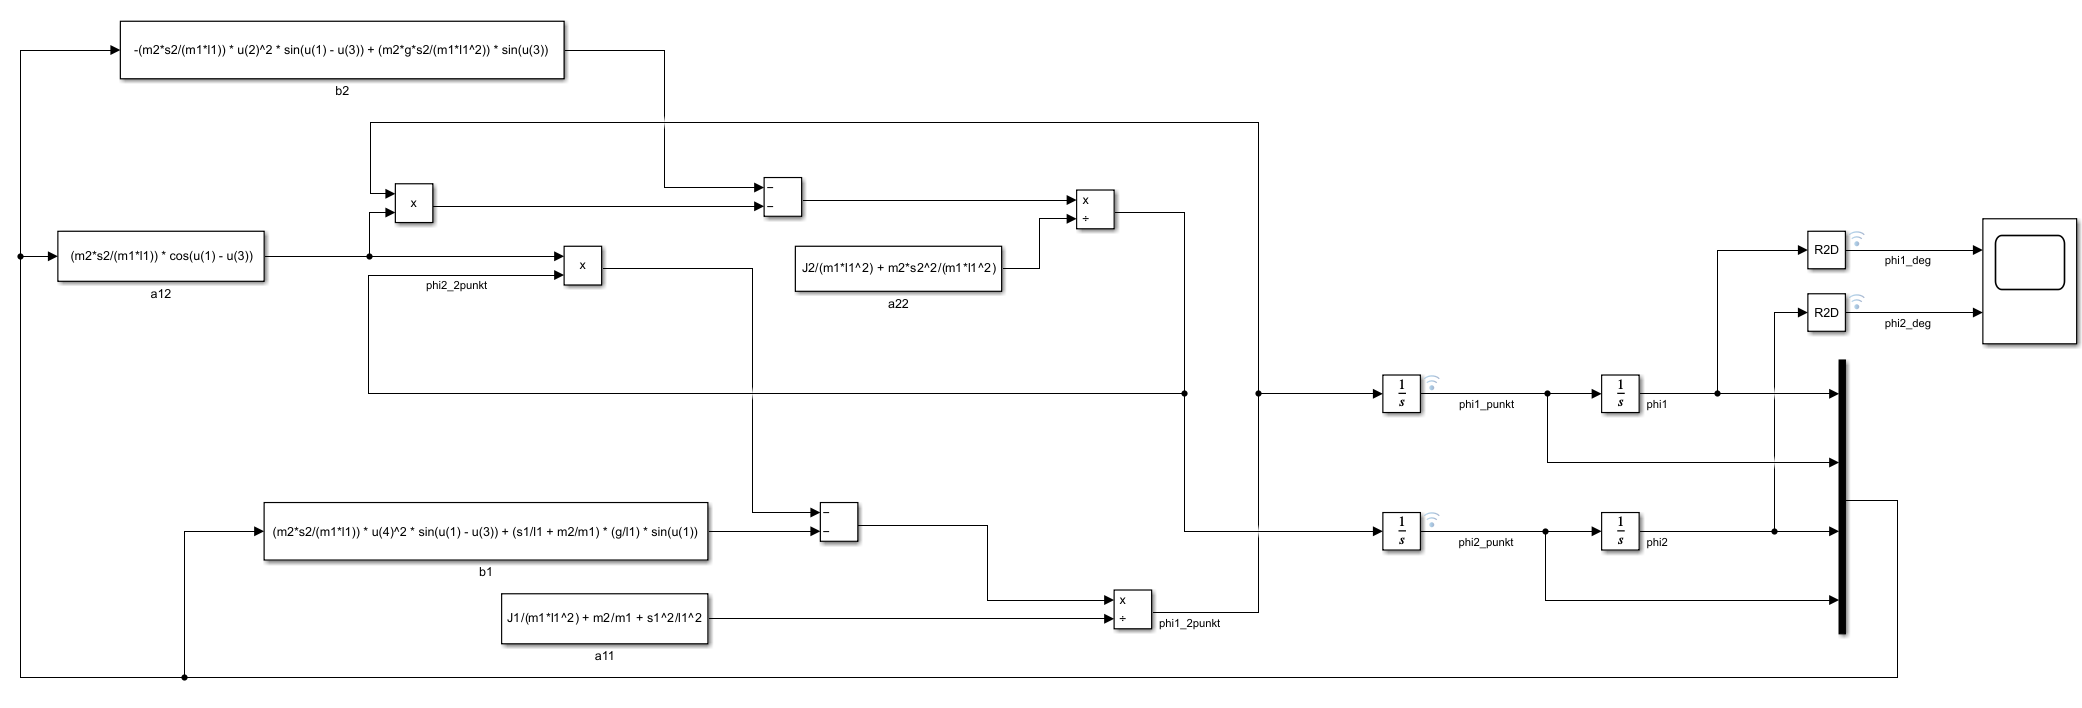
\includegraphics[width=1\textwidth]{figures/Blockschaltbild.png}
  \caption{Blockschaltbild des Doppelpendels}
  \label{fig:Blockschaltbild}
\end{figure}

\section{Simulation mit Zustandsraum}
\textbf{Linearisierung am Gleichgewichtspunkt}\\
Der Gleichgewichtspunkt ist definiert als:
\begin{align}
  \varphi_1 &= 0, &\dot{\varphi}_1 &= 0, &\varphi_2 &= 0, &\dot{\varphi}_2 &= 0
\end{align}

Zur Linearisierung werden hier die partiellen Ableitungen berechnet:
\begin{align}
  \frac{\partial b_1}{\partial \varphi_1} &= \left(\frac{s_1}{l_1} + \frac{m_2}{m_1}\right) \cdot \frac{g}{l_1} \cdot \cos(\varphi_1)\Big|_{\varphi_1=0} = \left(\frac{s_1}{l_1} + \frac{m_2}{m_1}\right) \cdot\frac{g}{l_1} \\
  \frac{\partial b_1}{\partial \varphi_2} &= 0 \\
  \frac{\partial b_1}{\partial \dot{\varphi}_1} &= 0 \\
  \frac{\partial b_1}{\partial \dot{\varphi}_2} &= 0 \\
  \frac{\partial b_2}{\partial \varphi_1} &= 0 \\
  \frac{\partial b_2}{\partial \varphi_2} &= \frac{m_2 \cdot g \cdot s_2}{m_1 \cdot l_1^2} \cdot \cos(\varphi_2)\Big|_{\varphi_2=0} = \frac{m_2 \cdot g \cdot s_2}{m_1 \cdot l_1^2} \\
  \frac{\partial b_2}{\partial \dot{\varphi}_1} &= 0 \\
  \frac{\partial b_2}{\partial \dot{\varphi}_2} &= 0
\end{align}

Aus den Ableitungen der Lagrange-Funktion $L$ ergeben sich weitere
partiellen Ableitungen, was in der folgenden Matrix $\mathbf{A}$
braucht. Das wird in m-Datei \codefile{Doppelpendel\_Linearisierung.m}
implementiert.

\textbf{Zustandsraumdarstellung}\\
Mit dem Zustandsvektor $\mathbf{x} = [\varphi_1, \dot{\varphi}_1, \varphi_2, \dot{\varphi}_2]^T$ wird das System in Zustandsraumdarstellung beschrieben:
\begin{align}
  \dot{\mathbf{x}} &= \mathbf{A}\mathbf{x} + \mathbf{B}\mathbf{u} \\
  \mathbf{y} &= \mathbf{C}\mathbf{x} + \mathbf{D}\mathbf{u}
\end{align}

Die Systemmatrix $\mathbf{A}$ wird konstruiert als:
\begin{align}
  \mathbf{A} = 
  \begin{bmatrix}
    0 & 1 & 0 & 0 \\
    \frac{\partial \ddot{\phi}_1}{\partial \phi_1} & \frac{\partial \ddot{\phi}_1}{\partial \dot{\phi}_1} & \frac{\partial \ddot{\phi}_1}{\partial \phi_2} & \frac{\partial \ddot{\phi}_1}{\partial \dot{\phi}_2} \\
    0 & 0 & 0 & 1 \\
    \frac{\partial \ddot{\phi}_2}{\partial \phi_1} & \frac{\partial \ddot{\phi}_2}{\partial \dot{\phi}_1} & \frac{\partial \ddot{\phi}_2}{\partial \phi_2} & \frac{\partial \ddot{\phi}_2}{\partial \dot{\phi}_2}
  \end{bmatrix}
\end{align}

Nachdem man m-Datei \codefile{Doppelpendel\_Linearisierung.m} durchgeführt hat, wird alle Matrizen berechnet. Schließlich wird die Blockschaltbild des Zustandsraummodells in der Abbildung \ref{fig:Blockschaltbild_Zustandsraum} gezeichnet und in slx-Datei \codefile{Doppelpendel\_Zustandsraum.slx} simuliert. Das Solver wird hier gleiche wie die Simulation mit 5-Punkte Schema eingestellt.
\begin{figure}[H]
  \centering
  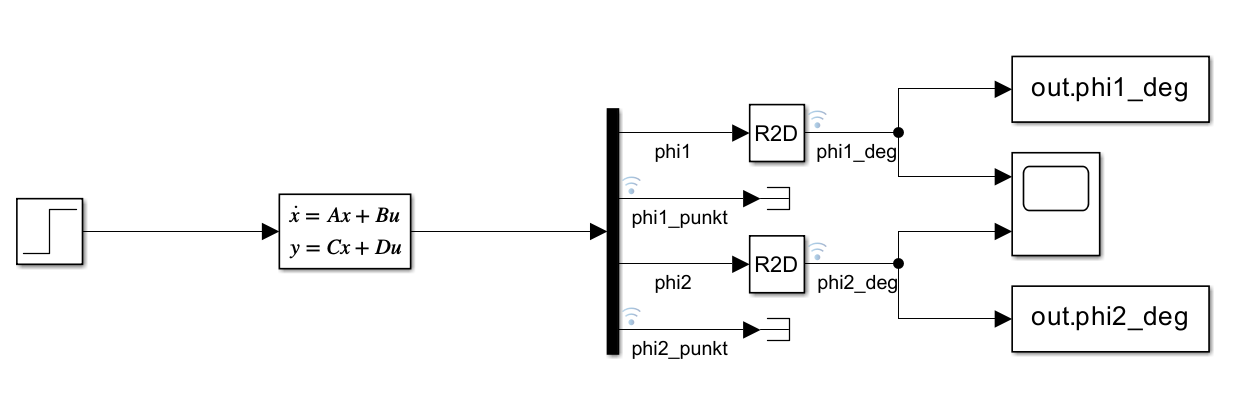
\includegraphics[width=0.7\textwidth]{figures/Blockschaltbild_Zustandsraum.png}
  \caption{Blockschaltbild des Zustandsraummodells}
  \label{fig:Blockschaltbild_Zustandsraum}
\end{figure}

\section{Simulation in Matlab (ohne Simulink)}
Das Skript erstellt von der gleichen Gleichungen, was die Simulation mit 5-Punkte Schema genutzt hat. Die Simulation wird in m-Datei \codefile{Doppelpendel.m} durchführen und die Funktion \codefile{xpunkt\_Doppelpendel.m} aufrufen, um die Differentialgleichung aufzustellen. Danach wird die Differentialgleichung mit \textit{ode15s} gelöst. Die Simulation wird mit den gleichen Parametern und Anfangsbedingungen wie die Simulation in Simulink durchführen. 

Hier werden die Simulation erweitert, um ein Dreifachpendel zu simulieren. Das kann man in der m-Datei \codefile{Dreifachpendel.m} durchführen. Die m-Datei \codefile{Dreifachpendel.m} wird die Funktion \codefile{xpunkt\_Dreifachpendel.m} aufrufen und mit ähnlichen Lösungsweisen wie die Simulation des Doppelpendels durchführen. 


\chapter{Simulationsergebnisse}\label{ch:Simulationsergebniss}

Die Abbildung \ref{fig:Doppelpendel_Ergebniss_Simulink} zeigt die Ergebnisse der Simulation des Doppelpendels in Simulink mit 5-Punkte Schema. Die Simulation wurde mit den Parametern $l_1 = 0,2~m$, $l_2 = 0,2~m$, $m_1 = 0,0295~kg$, $m_2 = 0,0295~kg$ und $s_1 = 0,1~m$, $s_2 = 0,1~m$, $J_1 = 9,8175 \cdot 10^{-5}~kg \cdot m^2$, $J_2 = 9,8175 \cdot 10^{-5}~kg \cdot m^2$ durchgeführt. Die Anfangswerte für die Winkel wurden auf $\varphi_1 = 0~rad$ und $\varphi_2 = \pi/2~rad$ gesetzt. Die Simulation wurde über einen Zeitraum von $10~sec$ durchgeführt.
\begin{figure}[H]
    \centering
    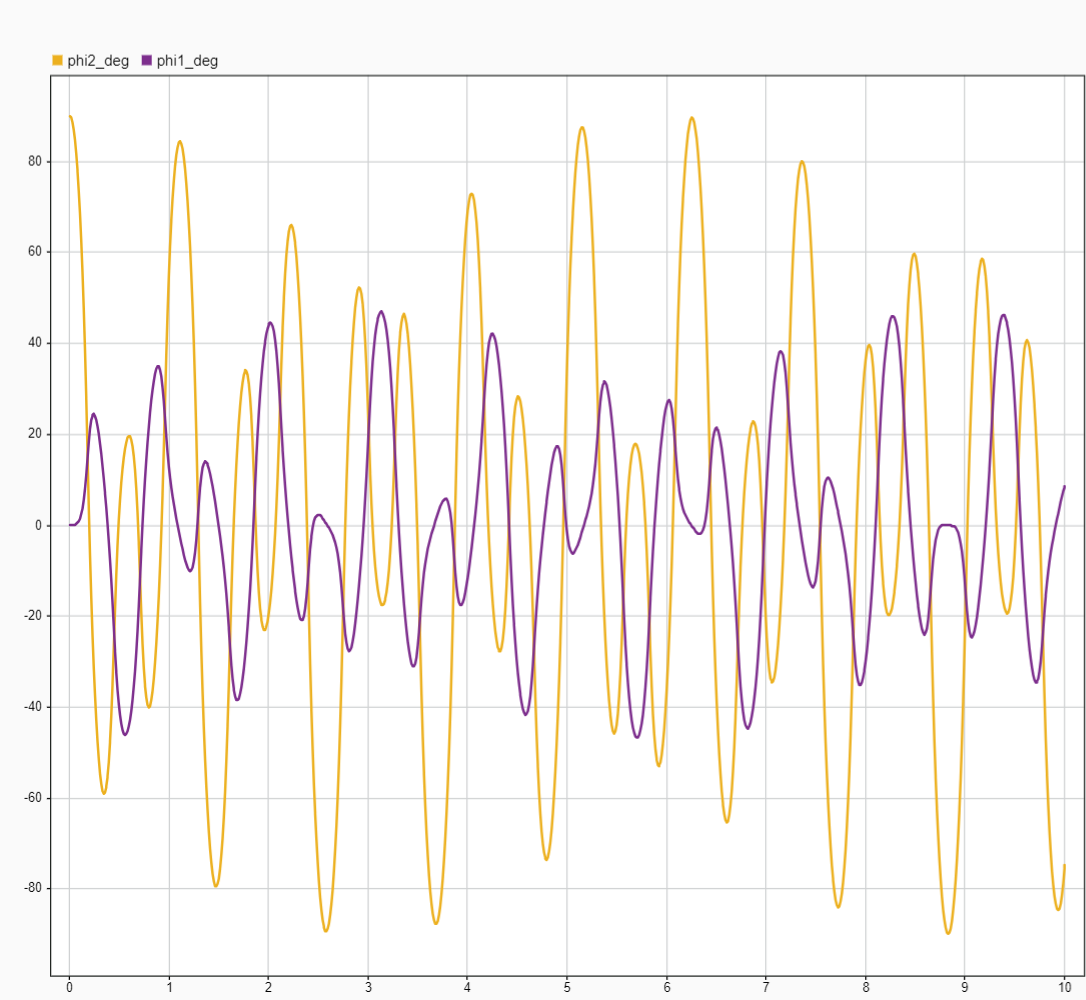
\includegraphics[width=0.45\textwidth]{figures/Doppelpendel_Ergebniss_Simulink.png}
    \caption{Doppelpendel Ergebniss mit 5-Punkte Schema}
    \label{fig:Doppelpendel_Ergebniss_Simulink}
\end{figure}

Die Abbildung \ref{fig:Doppelpendel_Ergebniss_Zustandsraum} zeigt die Ergebnisse der Simulation des Doppelpendels mit Zustandsraummodell. Die Simulation wurde mit den gleichen Parametern und Anfangsbedingungen wie die Simulation mit 5-Punkte Schema durchgeführt. Nach Linearisierung des Modells sieht die die Ergebnisse ähnlich aber nicht gleich wie die Ergebnisse der Simulation mit 5-Punkte Schema. 
\begin{figure}[H]
  \centering
  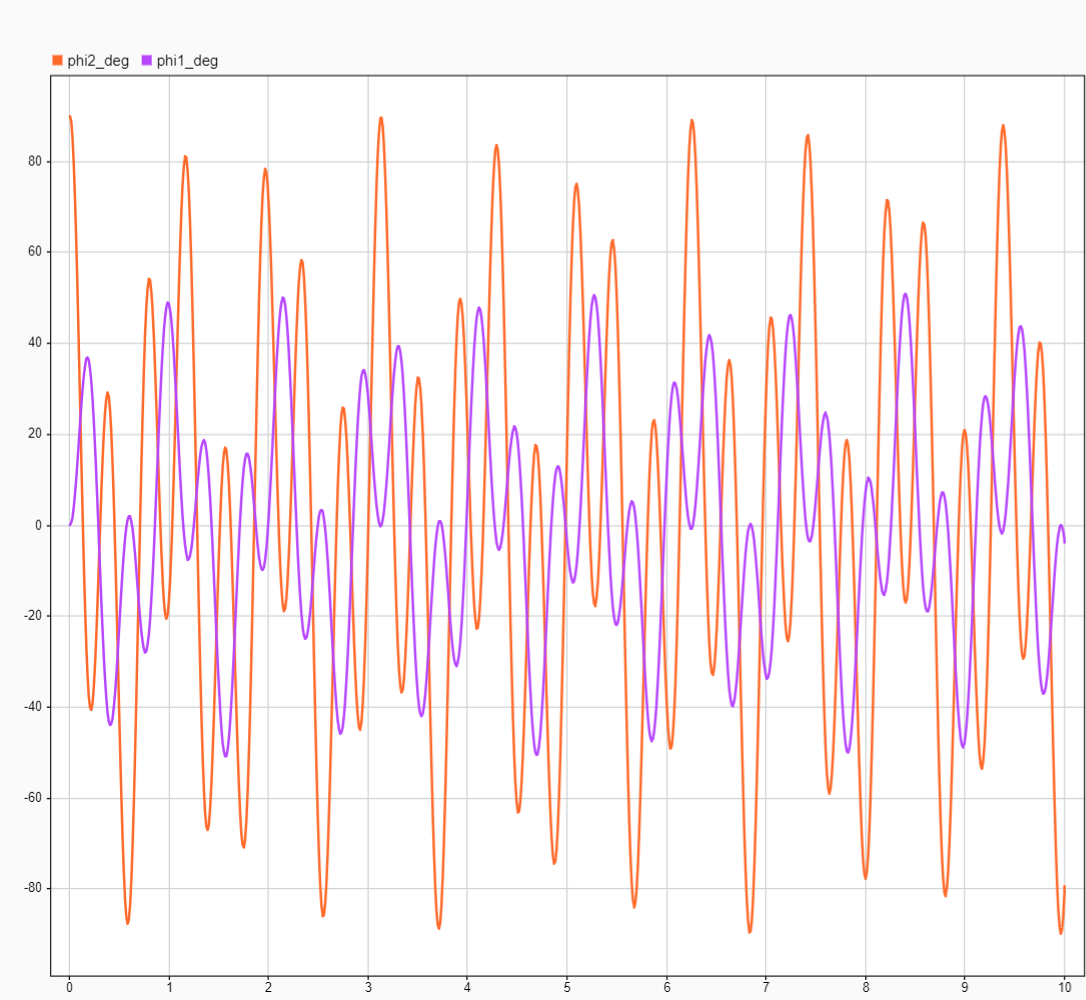
\includegraphics[width=0.45\textwidth]{figures/Doppelpendel_Ergebniss_Zustandsraum.png}
  \caption{Doppelpendel Ergebniss mit Zustandsraummodell}
  \label{fig:Doppelpendel_Ergebniss_Zustandsraum}
\end{figure}

Folgende Abbildung \ref{fig:Doppelpendel_Ergebniss} zeigt die Ergebnisse der Simulation des Doppelpendels in Matlab (ohne Simulink). Die Simulation wurde mit den gleichen Parametern und Anfangsbedingungen wie die Simulation in Simulink durchgeführt. Die Ergebnisse zeigen, dass die Simulation in Matlab fast gleiche Ergebnisse wie die Simulation in Simulink mit 5-Punkte Schema liefert. 
\begin{figure}[H]
    \centering
    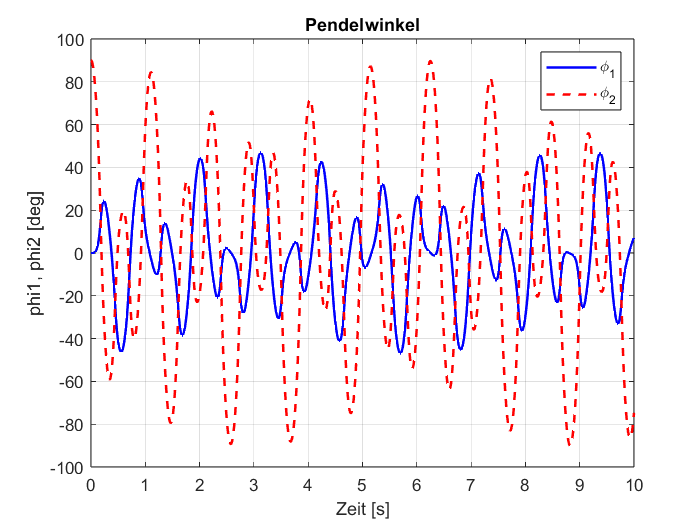
\includegraphics[width=0.6\textwidth]{figures/Doppelpendel_Ergebniss.png}
    \caption{Doppelpendel Ergebniss in Matlab (ohne Simulink)}
    \label{fig:Doppelpendel_Ergebniss}
\end{figure}

Für Erweiterungen simuliert hier ein Dreifachpendel mit Matlab (ohne Simulink). Die Abbildung \ref{fig:Dreifachpendel_Ergebniss} zeigt die Ergebnisse der Simulation des Dreifachpendels. Die Simulation wurde mit gleiche Parametern und wie das Doppelpendel durchgeführt. Die Anfangswerte für die Winkel wurden auf $\varphi_1 = 0~rad$, $\varphi_2 = 0~rad$ und $\varphi_3 = \pi/2~rad$ gesetzt. Die Abbildung \ref{fig:Dreifachpendel_Ergebniss_Trajektorie} zeigt die Trajektorie der dritten Pendel in der Simulation des Dreifachpendels.
\begin{figure}[H]
    \centering
    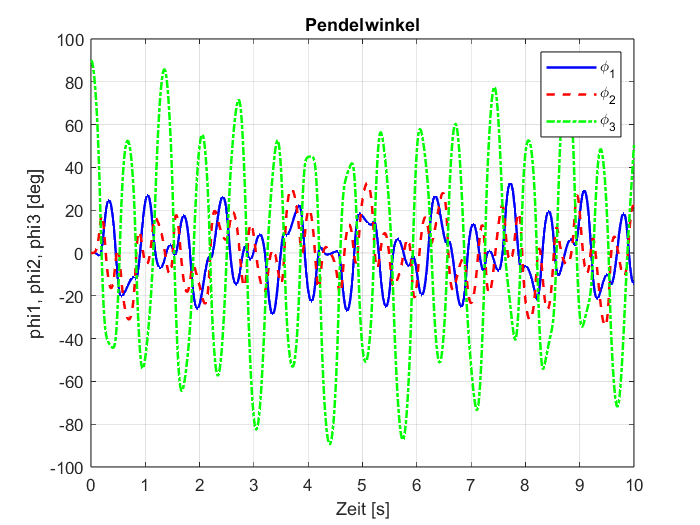
\includegraphics[width=0.6\textwidth]{figures/Dreifachpendel_Ergebniss.png}
    \caption{Dreifachpendel Ergebniss in Matlab (ohne Simulink)}
    \label{fig:Dreifachpendel_Ergebniss}
  \end{figure}

\begin{figure}[H]
    \centering
    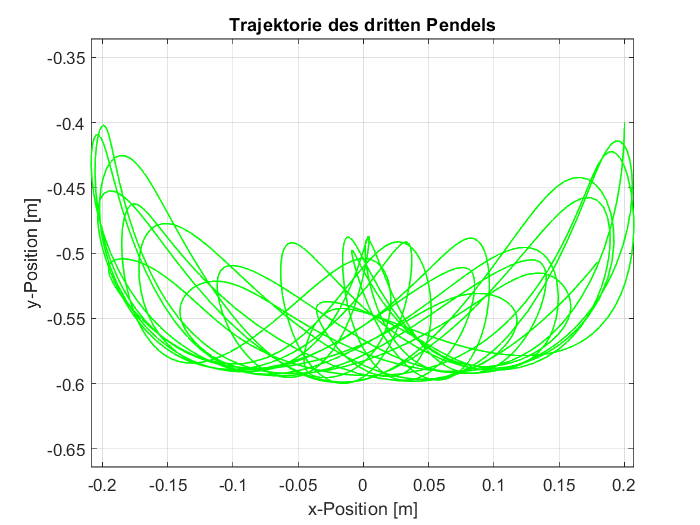
\includegraphics[width=0.6\textwidth]{figures/Dreifachpendel_Ergebniss_Trajektorie.png}
    \caption{Trajektorie von dritten Pendel des Dreifachpendels}
    \label{fig:Dreifachpendel_Ergebniss_Trajektorie}
\end{figure}

Die Ergebnisse der Simulation zeigen, dass das Doppelpendel und das Dreifachpendel chaotisches Verhalten aufweisen. Beide Methoden (Matlab und Simulink mit 5-Punkte Schema) liefern ähnliche Ergebnisse, wobei die Simulation mit Zustandsraummodell eine gewisse Abweichung aufweist. Der Grund für diese Abweichung könnte in der Linearisierung des Modells liegen, die nur in einem kleinen Bereich um den Gleichgewichtspunkt gültig ist. 

Zusammenfassend lässt sich sagen, dass die Simulation des Doppelpendels und des Dreifachpendels in Matlab und Simulink erfolgreich durchgeführt wurde. Die Ergebnisse bestätigen die theoretischen Annahmen über die Dynamik des Systems. Mit aktuellen Modellen und Methoden können in der Zukunft weitere Simulationen durchgeführt werden. Z.B. Regelung des Pendels mit PID-Regler oder Zustandsraumregelung. 
%\chapter*{Anhang}
\addcontentsline{toc}{chapter}{Anhang}



\bibliographystyle{ieeetr}
\bibliography{refs}

\end{document}
